\chapter{Theoretical Framework}
\label{ch:teo}

\begin{chapterquote}{Herbert Simon}
Human beings, viewed as behaving systems, are quite simple.
The apparent complexity of our behavior over time is largely a
reflection of the complexity of the environment in which we find
ourselves.
\end{chapterquote}


\section{Machine Learning}

The process of learning has long fascinated people from many different disciplines such as psychology, biology, neuroscience, computer science, statistics, mathematics, physics etc. However, it has been difficult to agree upon a precise definition of the process mainly because it depends on the viewpoint. Since this work is motivated on the desire to make computers think and act like human beings, one alternative would be a brain simulation. Unfortunately, brain simulation faces two main obstacles[MLT]:
\begin{enumerate}
\item  The detailed structure of the brain is not known yet
\item Even if we knew the detailed structure of the brain, it does not exist a fast enough computer to simulate it.
\end{enumerate}

Thus, the aim is to construct models that imitate a specific and limited behavior of humans. In this case, the behavior is the generation of a natural language such as English or Spanish. On the other hand, since what we have is data, the key concept to think is learning from data. Finally, if we put it on human behavioral terms the key concept is learning from experience[MLA]. 

Therefore, machine Learning is about making computers modify or adapt their actions so that these actions get more accurate, where accuracy is measured by how well the chosen actions reflect the correct ones[MLA].As there are several ways to achieve this task there are different types of machine learning explained as follows [MLA]:

\begin{itemize}
\item \textbf{Supervised Learning} It is said that it is supervised learning when a training set of examples with the correct responses or targets are provided and, based on this training set, the algorithm generalises to respond correctly to all possible inputs.

\item \textbf{Unsupervised Learning} The algorithm tries to identify similarities between the inputs so that the inputs that have something in common are categorised together. In this type of learning correct responses are not provided.

\item \textbf{Reinforcement Learning} The algorithm gets told when the answer is wrong but does not get told how to correct it. Instead, it has to explore and try out different possibilities until it works out how to get the right answer. 

\item \textbf{Evolutionary learning} In this type of learning, biological evolution is seen as a learning process where the organisms adapt to improve their survival rates and chance of having offspring in their environment. It uses an idea of fitness which corresponds to a score for how good the solution is. 
\end{itemize}

\subsection{Overfitting}
\subsection{Underfitting}

\section{McCulloch and Pitts Neurons}
McCulloch and Pitts modeled a neuron as a mathematical model in order to extract only the essentials required to accurately represent the entity, removing all the obscured details. They took in account three basic elements: a set of weighted inputs ($w_i$), an adder that sums the input signals, and an activation function that decides if the neuron fires to the current inputs.
\begin{figure}[h]
\centering
 
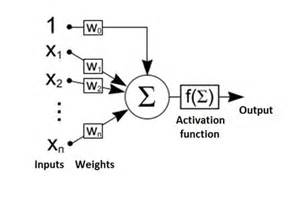
\includegraphics[width=10cm,height=5cm]{model_of_neuron.jpg}
\caption{McCulloch and Pitt's Neuron Model}
\label{fig:neuron}
\end{figure}

Hence, when all signals arrive into our neuron, they are added to determine if it should be activated, meaning if the sum is greater than the threshold $\theta$. The mathematical expression is as follows:\\
\begin{equation} \label{eq:neuron}
h=\sum_{i=1}^{m} w_i * x_i
\end{equation}\ref{eq:neuron}

Thus the output of the neuron is nothing more than the sum of the $m$ inputs ($x_i$) multiplied by the weights ($w_i$). Furthermore, units can be given biases by introducing an extra input to each unit which always have a value of 1. The weight on this extra input is called the bias and is equivalent to a threshold of the opposite sign \cite{polk2002cognitive}.


\section{Neural Networks}

A simple neural network is shown in Figure \ref{fig:nn}. It is formed by input units at the bottom, any number of intermediate layers (called hidden layers), where each of the units are  defined as a McCulloch and Pitts neuron and a layer of output units at the top. Connections within a layer from a higher to lower layers are forbidden. 

The point of a neural network is to discover the best weights for the weighted connections, since they are unknown. 

Learning or training refers to finding a set of weights that ensure that for each input vector, the output vector produced by the network is sufficiently close to the desired output vector \cite{polk2002cognitive}. This means, we need to compare the error defined as the difference between the actual and desired output vectors for every case.

Then to adjust the weights the error E in equation \ref{eq:error} is multiplied by a parameter called the learning rate $\nu$ and by the input $x_i$. Then this value is added to the weight ($w_ij$) for each j neuron and input i.

\begin{equation}
\label{eq:error}
E=(t_j - y_i)
\end{equation}
\begin{equation}
\label{eq:weight}
w_ij \leftarrow w_ij+\nu E * x_i
\end{equation} where $0>=\nu<=1$ \\
\ref{eq:weight}
\begin{figure}
\label{fig:nn}
\center
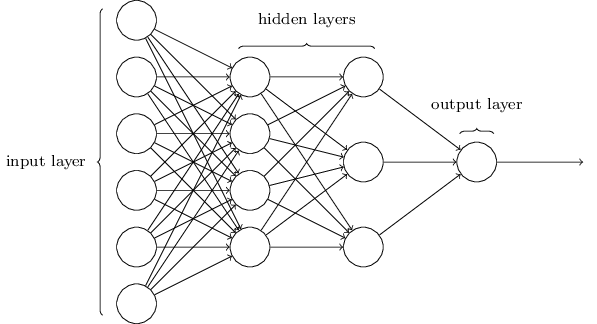
\includegraphics[width=10cm,height=5cm]{NN.jpg}
\caption{Neural Network}
\end{figure}
\\
Although the first time the network might get some answers correct and some wrong, the next time it is expected to improve until eventually its performance stop improving. How much the weights are changed is controlled by the learning rate $\nu$. If it is too big, the weights will change a lot  making the network unstable so that it never settles down. On the other hand, if $\nu$ is too short it will be stable and resistant to errors and inaccuracies in the data, but it will take too long to learn. Hence, the typical earning rate is between 0.1 and 0.4 [MLA].

\subsection{Backpropagation}

As explained before, the weight vector is formed by the internal adjustable parameters which are adjusted to minimize the error E showed in equation \ref{eq:error}	. To achieve this task the gradient descent is used. Therefore, it is necessary to compute the partial derivative of E with respect to each weight in the network (\ref{eq:der}). This indicates by what amount the error would increase or decrease if the weight were increased by a tiny amount. Then, the weight vector is adjusted in the opposite direction to the gradient vector \cite{lecun2015deep}. 

\begin{equation}
\label{eq:der}
x=1
\end{equation}

The backpropagation procedure to compute the gradient of an objective function with respect to the weights of a multilayer stack of modules is nothing more than a practical application of the chain rule for derivatives. The key insight is that the derivative (or gradient)
of the objective with respect to the input of a module can be computed by working backwards from the gradient with respect to the output of that module (or the input of the subsequent module). \cite{lecun2015deep}

Falta poner las ecuaciones!!!!



Using equation (z) we can compute dE/dy for any unit in the penultimate layer when given dE/dy for all units n the last layer \cite{polk2002cognitive}. Therefore,we can repeat this procedure to compute this term for successively earlier layers, computing dE/dw for the weights to go. 


It was commonly thought that simple gradient descent would get trapped in poor local minima but in practice, poor local minima is rarely a problem with large networks.\cite{lecun2015deep}


After training, the performance of the system is measured on a different set of examples called a test set. This serves to test the generalization ability of the machine\cite{lecun2015deep}.

\section{Deep Learning}

Representation learning is a set of methods that allows a machine to be fed with raw data and to automatically discover the representations needed for detection or classification. Deep-learning methods are representation-learning methods with multiple levels of representation. With the composition of enough such transformations, very complex functions can be learned. For classification tasks, higher layers of representation amplify aspects of the input that are important for discrimination and suppress irrelevant variations\cite{lecun2015deep}.

\section{Sequential Data}
For sequential data, it is not allowed to make the assumption that data is independent and identically distributed (i.i.d.). Meaning, we are not allowed to express the likelihood function as the product over all data points of the probability distribution evaluated at each point.
Sequential data often arise through measurement of time series, for example the rainfall measurements on successive days at a particular location., or the daily values of a currency exchange rate, or the acoustic features at a successive time frames used for speech recognition. 

Sequential data can also arise in contexts other than time series such as the sequence of nucleotide base pairs along a strand of DNA or the sequence of characters in a an English sentence.

For convenience, we shall sometimes refer to past and future events in a a sequence
[PRML]
-----------------------------------------

\subsection{Recurrent Neural Networks}
A recurrent neural network is a artificial neural network model.The difference of its structure is that connections among hidden units associated with a time delay are allowed, enabling the model to retain information about the past inputs. In this way, temporal correlations between events that are possibly far away from each other in the data can be discovered \cite{pascanu2013difficulty}. 

The network is `deep' in both space and time, in the sense that every piece of information passing either vertically or horizontally through the computation graph will be acted on by multiple successive weight matrices and nonlinearities \cite{graves2013generating}.

RNNs are fuzzy in the sense that they use their internal representation to perform a high-dimensional interpolation between training examples so they do not use exact temples from the training data to make predictions \cite{graves2013generating}
The result is that rnns synthesise and reconstitute the training data in a complex way, and rarely generate the same thing twice. Furthermore, fuzzy predictions do not suffer from the curse of dimensionality, and are therefore much better at modelling real-valued or multivariate data than exact matches  \cite{graves2013generating}.

For tasks that involve sequential inputs, such as speech and language, it results better to use RNNs. RNNs process an input sequence one element at a time, maintaining in their hidden units a ‘state vector’ that implicitly contains information about the history of all the past elements of the sequence.\cite{lecun2015deep}


\subsubsection{Backpropagation Through Time}

RNNs, once unfolded in time (Fig. 5), can be seen as very deep feedforward networks in which all the layers share the same weights\cite{lecun2015deep}
One approach to compute the gradients is Backpropagation Through Time (BPTT). Here, the model is presented as a deep multi-layer one where backpropagation is applied on the unrolled model\cite{pascanu2013difficulty}.


\subsubsection{RNS Training Issues}
RNNs are very powerful dynamic systems, but training them has proved to be problematic because the backpropagated gradients either grow or shrink at each time step, so over many time steps they typically explode or vanish\cite{lecun2015deep}

The exploding gradients problem refers to the large increase in the norm of the gradient during training caused by the explosion of the long term components. On the other hand, the vanishing gradients problem is presented when long term components go exponentially fast to norm 0 making impossible for the model to learn correlation between temporally distant events \cite{pascanu2013difficulty}. 

\subsubsection*{The exploding gradients problem }

 One simple mechanism to deal with the exploding gradients problem is to rescale them whenever they go over a threshold. One good heuristic for setting this threshold is to look at statistics on the average norm over a sufficiently large number of updates. In this way, we can handle very abrupt changes in norm, so the algorithm can be thought of as adapting the learning rate based on the norm of the gradient  \cite{pascanu2013difficulty}.
Algorithm
\subsubsection*{The vanishing gradients problem}

The vanshing gradients problem makes it difficult to learn to store information for very long. 
This amnesia makes them prone to instability when generating sequences. The problem is that if the network's predictions  are only based on the last few inputs, and these inputs were themselves predicted by the network, it has little opportunity to recover from past mistakes. Having a longer memory has a establishing effect, because even if the network cannot make sense of its recent history, it can look further back in the past to formulate its predictions. \cite{graves2013generating}

A solution proposed for the vanishing gradient problem is to use a regularization term that forces the error signal not to vanish as it travels back in time  write the algorithm 1 and the regularization term \cite{pascanu2013difficulty}.
A second idea is to augment the network with an explicit memory. The first proposal of this kind is the long short-term memory (LSTM) networks.


\subsubsection{Long Short-Term Memory Networks}
Long Short-term Memory (LSTM) is an RNN architecture designed to be better at storing and accessing information than standard RNNs \cite{graves2013generating}.
Although in most RNNs the hidden layer function H is an elementwise application of sigmoid function.,  Long Short-Term Memory  architecture uses purpose-built memory cells to store information, is better at finding and exploiting long range dependencies in the data. It has a input gate, forget gate, output gate, cell and cell input activation vectors, all of which are the same size as the hidden vector h. \cite{graves2013generating}
The memory cell (hay que ver cual de las 3 es) acts like an accumulator or a gated leaky neuron: it has a connection to itself at the next time step that has a weight of one, so it copies its own real-valued state and accumulates the external signal, but this self-connection is multiplicatively gated by another unit that learns to decide when to clear the content of the memory \cite{lecun2015deep}.

LSTM networks have subsequently proved to be more effective than conventional RNNs, especially when they have several layers for each time step\cite{lecun2015deep}.
The full gradient can be calculated with backpropagation through time \cite{graves2013generating}
This model has been used in several applications such as speech and handwriting recognition.\cite{graves2013generating}



\section{Language Modelling}
\subsection{N-grams}
The standard approach to statistical modelling of language was based on counting frequencies of occurrences of short symbol sequences of length up to N (called N-grams). The number of possible N-grams is on the order of VN, where V is the vocabulary size N-grams treat each word as an atomic unit, so they cannot generalize across semantically related sequences of words, whereas neural language models can because they associate each word with a vector of real valued features, and semantically related words end up close to each other in that vector space (Fig. 4).\cite{lecun2015deep}

\subsection{Prediction by Partial Matching}
The prediction by partial algorithms are compression algorithms where the prediction is determined by counting exact matches between the recent history and the training set \cite{graves2013generating}.
    
\subsection{Neural Language Models}
Before the introduction of neural language model the standard approach to statistical modelling of language did not exploit distributed representations\cite{lecun2015deep}

Recurrent Neural Networks are dynamic models that have been used to generate sequences in different domains such as music, text and motion capture data \cite{graves2013generating}.
They also have been found to be very good at predicting the next character in the text or the next word in a sequence, since the hidden layers of a multilayer neural network learn to represent the network’s inputs in a way that makes it easy to predict the target outputs.\cite{lecun2015deep}

Novel sequences can be generated by by a trained network by iteratively sampling from the network's output distribution, assuming the predictions are probabilistic and then feeding in the sample as input at the next step, meaning by making the network treats its inventions as if they were real. 
\cite{graves2013generating}.


\subsection{Text Representation}
Text data is discrete, and is typically presented to neural networks using `onehot' input vectors. That is, if there are K text classes in total, and class k is fed in at time t, then xt is a length K vector whose entries are all zero except for the kth, which is one. Pr(xt+1jyt) is therefore a multinomial distribution, which can be naturally parameterised by a softmax function at the output layer:
formulas

\subsubsection{Word-level language modelling}

In most cases, text prediction  is performed at the word level. K is therefore the number of words in the dictionary. \cite{graves2013generating}
In the first layer, each word creates a different pattern of activations, or word vectors (Fig. 4). In a language model, the other layers of the network learn to convert the input word vectors into an output word vector for the predicted next word, which can be used to predict the probability for any word in the vocabulary. Learning word vectors turned out to also work very well when the word sequences come from a large corpus of real text and the individual micro-rules are unreliable.\cite{lecun2015deep}

This can be problematic for realistic tasks, where the number of words often exceeds 100,000. As well as requiring many parameters to model, having so many classes demands a huge amount of training data to adequately cover the possible contexts for the words. A further diculty is the high computational cost of evaluating all the exponentials during training. Furthermore, word-level models are not applicable to text data containing non-word strings, such as multi-digit numbers or web addresses.\cite{graves2013generating}
\subsubsection{Character-level language modelling}

Character-level language modelling has been found to give slightly worse performance than equivalent word-level models. Nonetheless, predicting one character at a time is more interesting from the perspective of sequence generation, because it allows the network to invent novel words and strings.
\cite{graves2013generating}

